%%%%%%%%%%%%%%%%%%%%%%%%%%%%%%%%%%%%%%%%%%%%%%%%%%%%%%%%%%%%%%%%%
% Tese de Doutorado / Dept Fisica, CFM, UFSC                    %
% Andre@UFSC - 2014                                             %
%%%%%%%%%%%%%%%%%%%%%%%%%%%%%%%%%%%%%%%%%%%%%%%%%%%%%%%%%%%%%%%%%

%:::::::::::::::::::::::::::::::::::::::::::::::::::::::::::::::%
%                                                               %
%                          Capítulo 3                           %
%                                                               %
%:::::::::::::::::::::::::::::::::::::::::::::::::::::::::::::::%

%***************************************************************%
%                                                               %
%                            PyCASSO                            %
%                                                               %
%***************************************************************%

\chapter{PyCASSO}
\label{sec:pycasso}

A fim de agilizar o desenvolvimento de ferramentas de manipulação de cubos de
dados do CALIFA, alguns programas de computador foram desenvolvidos. Foi montado
um ``kit de ferramentas'', chamado PyCASSO ({\em Python CALIFA} \starlight\ {\em
Synthesis Organizer}), para organizar e analisar o resultado da síntese de
populações sobre os dados do CALIFA. PyCASSO foi desenvolvido em sua maior parte
pelo autor desta tese, utilizando a linguagem Python, e foi utilizado de forma
extensiva pelo grupo de populações estelares (cerca de 10 pessoas), resultando
em vários artigos, alguns deles descritos neste capítulo.

A grosso modo, PyCASSO é composto de três partes:

\begin{enumerate}

\item Conversor de tabelas. Com ele se converte a saída do \starlight (arquivos
ASCII para cada pixel de cada galáxia) para cubos de dados nos formatos FITS e
HDF5, de forma a otimizar o acesso aos dados. Uma galáxia leva tipicamente 2
minutos para ser carregada em memória usando arquivos texto. Este tempo se reduz
para menos de um segundo usando arquivo FITS. Há outra otimização para acessar
dados de várias galáxias simultaneamente, utilizando o formato HDF5. Neste caso
a carga dos dados em disco para a memória é ``preguiçosa'', quer dizer, é feita
somente quando os dados são efetivamente acessados.

\item Camada de entrada e saída. Os arquivos FITS e HDF5 foram montados de forma
a serem facilmente acessados em qualquer ambiente. Ainda assim, há uma camada de
abstração de armazenamento, onde as várias matrizes e cubos são acessadas com
nomes próprios (por exemplo, \texttt{popx}, que designa a fração de luz
distribuída pelas populações estelares), de forma a ser possível programar
ferramentas de análise sem precisar se preocupar com as características de cada
formato de armazenamento.

\item Camada de análise. Como foi mencionado na Seção \ref{sec:Intro:Sintese}, o
resultado da síntese consiste em cubos indexados por zona. Os dados ficam
armazenados no disco desta forma. Porém, na grande maioria das vezes se está
interessado na informação espacialmente resolvida. Esta camada implementa uma
rotina de conversão da notação de zonas para $(x, y)$. Boa parte das
propriedades da síntese, como luminosidade, massa, atenuação por poeira, e idade
estelar, já estão implementadas. Estes cubos espacialmente resolvidos são
calculados dinamicamente, quer dizer, não ocupam memória do sistema até que
sejam acessados. Existem outras rotinas para calcular geometria, perfis radiais
e azimutais, e raio de escala. Outras rotinas podem ser adicionadas
facilmente\footnote{Há um estudo de PCA (análise de componentes principais)
sendo desenvolvido pelo estudante da UFSC Eduardo A. D. Lacerda, por
exemplo.}.

\end{enumerate}

Este software está sendo utilizado pelo grupo de populações estelares da
colaboração do CALIFA, do qual o autor faz parte. No total são aproximadamente
10 pessoas utilizando este software. Foram publicados 6 artigos que utilizam
extensivamente PyCASSO, e mais alguns que utilizaram algum dado resultante de
forma indireta, apresentados na Seção \ref{sec:pycasso:art}.


%***************************************************************%
%                                                               %
%                     PyCASSO - Ferramenta                      %
%                                                               %
%***************************************************************%

\section{A ferramenta de manipulação de cubos de dados PyCASSO}
\label{sec:pycasso:Pycasso}

PyCASSO é uma biblioteca desenvolvida em Python. Porém uma biblioteca não é nada
sem uma boa documentação. Aqui se apresenta de forma breve das capacidades do
PyCASSO. A documentação completa se encontra no Apêndice \ref{apendice:manual}.

O trabalho com a variedade e quantidade de dados gerados pela síntese espectral
em 3-D tem em geral um caráter fortemente exploratório. Frequentemente não se
sabe exatamente o que se está buscando, e o trabalho do programador/cientista
consiste em desenhar gráficos, realizar cálculos, determinar operações ou
filtros nos dados com base nestes gráficos e cálculos, desenhar novamente, e
assim sucessivamente. Assim se escolheu a linguagem Python, que possui
ferramentas adequadas à programação exploratória\footnote{Além de estar se
tornando uma espécie de {\em lingua franca} na Astrofísica computacional.}, como
o \texttt{IPython}\footnote{\url{http://ipython.org/}} e o
\texttt{matplotlib}\footnote{\url{http://matplotlib.org/}}. Foi feito um esforço
para que o acesso aos dados de cada galáxia fosse feito de forma simples e
direta. Um exemplo de código pode ser visto na listagem de código fonte abaixo.

\begin{lstlisting}[language=Python, label={lst:dataAccess}, caption={Exemplo de
acesso aos dados. Todas as propriedades estão disponíveis diretamente pelo nome,
inclusive utilizando a função autocompletar da maioria dos ambientes de
desenvolvimento Python.}]
# Carregar arquivo FITS com os dados.
from pycasso import fitsQ3DataCube
K = fitsQ3DataCube('K0001_synthesis_suffix.fits')

# Acessar a idade media ponderada pela luminosidade.
at = K.at_flux__z

# Calcular a idade media da galaxia.
at_total = (at * K.Lobn__z).sum() / K.Lobn__z.sum()
print 'Idade media da galaxia: %.2f' % at_total
\end{lstlisting}

% FIXME: Rogério - Como chegas ao cubo de síntese? o pycasso passa o cubo para o
% starlight?

Para algumas operações, como o cálculo da idade estelar média feito na Figura
\ref{lst:dataAccess}, pode-se utilizar apenas o resultado para as zonas. Neste
caso, a idade estelar média é calculada usando a expressão $\langle \log t
\rangle^{\mathrm{gal}}_L = \sum_z \langle \log t \rangle_{L,z} L_z / \sum_z
L_z$, onde $L_z$ é a luminosidade de cada zona e $\langle \log t \rangle_{L,z}$
é a idade estelar média de cada zona. Entretanto, para tirar vantagem das
informações espaciais, é preciso converter as propriedades da notação de zona
para imagem.
Por exemplo, o programa a seguir calcula a idade estelar média espacialmente
resolvida\footnote{O mapa de idade já está previamente calculado, disponível
através da propriedade \texttt{at\_flux\_\_yx}. Esta conversão é feita
explicitamente aqui para ilustrar como a conversão pode ser feita para qualquer
propriedade.}, e em seguida desenha um gráfico da imagem gerada.

\begin{lstlisting}[language=Python, caption={Programa para desenhar o mapa de
idade estelar média ponderada pela luminosidade. O gráfico resultante é mostrado
na Figura \ref{fig:mapaIdade}.}, label={lst:mapaIdade}]
# Carregar arquivo FITS com os dados.
from pycasso import fitsQ3DataCube
K = fitsQ3DataCube('K0001_synthesis_suffix.fits')

# Converter zonas para imagem.
at_image = K.zoneToYX(K.at_flux__z, extensive=False)

# Desenhar o mapa.
import matplotlib.pyplot as plt
plt.imshow(at_image)
plt.colorbar()
\end{lstlisting}

\begin{figure}
	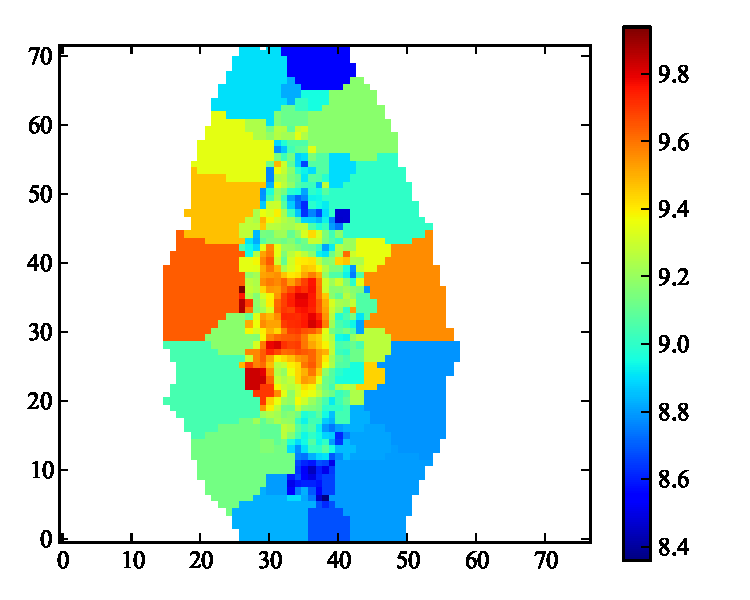
\includegraphics{figuras/mapa-idade}
	\caption[Mapa da idade estelar média da galáxia IC 5376] {Mapa de idade estelar
	média ponderada pela luminosidade da galáxia IC 5376, desenhado pelo programa
	da Listagem de código fonte \ref{lst:mapaIdade}.}
	\label{fig:mapaIdade}
\end{figure}

Enquanto um mapa é uma forma muito boa de visualizar informações em duas
dimensões, há vezes em que uma visualização resumida é mais adequada. Galáxias
em geral têm simetria aproximadamente axial, logo poder medir perfil radial das
propriedades das galáxias é fundamental para estudá-las. Com o PyCASSO, o
cálculo do perfil radial é bastante simples, como pode ser visto na Listagem de
código fonte \ref{lst:radprofIdade}, que calcula o perfil radial da idade
estelar média. O resultado está na Figura \ref{fig:radprofIdade}.

\begin{lstlisting}[language=Python, caption={Programa para desenhar o perfil
radial da idade estelar média ponderada pela luminosidade.},
label={lst:radprofIdade}]
# Carregar arquivo FITS com os dados.
from pycasso import fitsQ3DataCube
K = fitsQ3DataCube('K0001_synthesis_suffix.fits')

# Converter zonas para imagem.
at_image = K.zoneToYX(K.at_flux__z, extensive=False)

# Calcular o perfil radial.
bins = np.arange(0, 26, 1)
bin_center = (bins[1:] + bins[:-1]) / 2.0
at_rad = K.radialProfile(at_image, bins, rad_scale=1.0)

# Desenhar o perfil radial.
import matplotlib.pyplot as plt
plt.plot(bin_center, at_rad)
\end{lstlisting}

\begin{figure}
	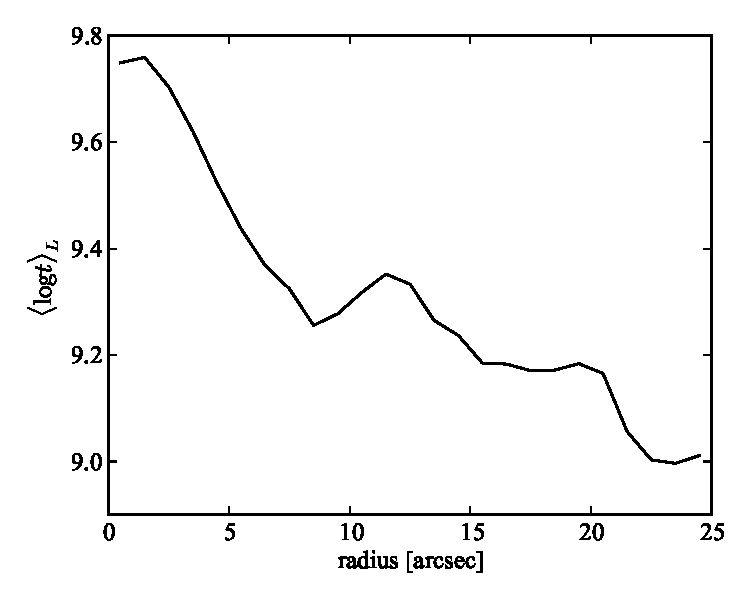
\includegraphics{figuras/radprof-idade}
	\caption[Perfil radial da idade estelar média da galáxia IC 5376] {Perfil
	radial da idade estelar média ponderada pela luminosidade da galáxia IC
	5376, desenhado pelo programa da Listagem de código fonte
	\ref{lst:radprofIdade}.}
	\label{fig:radprofIdade}
\end{figure}

Esta é só uma pequena demonstração das ferramentas existentes no PyCASSO. Também
é possível trabalhar com espectros, calcular perfis azimutais, lidar com {\em
pixels} mascarados, entre outras coisas. Tudo isto está descrito em detalhes no
manual do programa (Apêndice \ref{apendice:manual}).


%***************************************************************%
%                                                               %
%                      PyCASSO - Artigos                        %
%                                                               %
%***************************************************************%

\section{Artigos publicados}
\label{sec:pycasso:art}

Nesta seção discutem-se os artigos onde se utilizou PyCASSO e nos quais o autor
desta tese teve uma colaboração importante. Além destes artigos,
\citet{Husemann2013}, no artigo apresentando o DR1 do CALIFA, utiliza as massas
estelares determinadas pelo \starlight e disponibilizadas pelo PyCASSO para
caracterizar a amostra do CALIFA. O artigo que apresenta o DR2, de
\citet{GarciaBenito2015}, também utiliza as massas da mesma forma (ver Figura
\ref{fig:DRMass}). O mesmo artigo inclui a medição da PSF do CALIFA (ver Figura
\ref{fig:DR2PSF}), apresentado neste trabalho na Seção \ref{sec:psf:medida}.

\citet{GonzalezDelgado2014b} explora a relação massa--metalicidade estelar em
300 galáxias do CALIFA, utilizando PyCASSO. Em \citet{GonzalezDelgado2015} se
utiliza, além do PyCASSO, a decomposição bojo--disco (ver Seção
\ref{sec:morph:comp:bd}) em uma amostra de galáxias, realizada pelo autor desta
tese, adaptando técnicas discutidas no Capítulo \ref{sec:Decomp}.


%***************************************************************%
%                                                               %
%       PyCASSO - Resolving galaxies in Space and Time I        %
%                                                               %
%***************************************************************%

\subsection{Artigo: {\em Resolving galaxies in time and space. I. Applying
STARLIGHT to CALIFA datacubes}}
\label{sec:pycasso:art:Resolving1}

Este artigo por \citet{CidFernandes2013} descreve todo o processo de síntese
espectral dos cubos de dados do CALIFA, mencionados no Capítulo \ref{sec:intro},
e serve como uma demonstração da capacidade do PyCASSO. O artigo está
reproduzido na íntegra no Apêndice \ref{apendice:PaperResolving1}. O
preprocessamento dos cubos de espectros é feito através do programa QBICK,
desenvolvido por Rubén García Benito especialmente para o CALIFA, mas é genérico
o bastante para ser usado em outros cubos de dados. Após explicar em detalhes
todos os passos envolvidos desde o preprocessamento, passando pela descrição do
\starlight até a importação dos dados pelo PyCASSO, o artigo apresenta um caso
de estudo com a galáxia NGC 2916.

\begin{figure}
	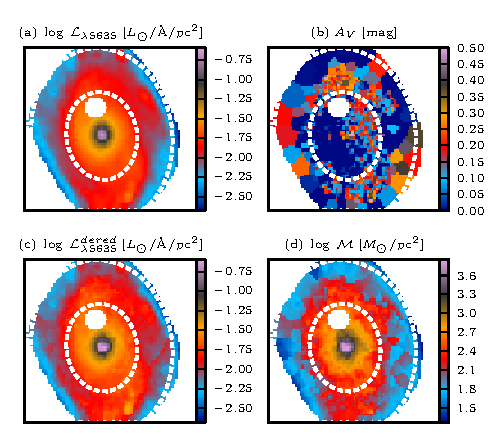
\includegraphics{figuras/L-M-AV-K0277}
	\caption[Propriedades físicas espacialmente resolvidas para a galáxia NGC
	2916] {Propriedades físicas espacialmente resolvidas para a galáxia NGC 2916. (a)
	Luminosidade em $5635\,\angstrom$ por unidade de área. (b) Atenuação por
	poeira na banda $V$. (c) Luminosidade em $5635\,\angstrom$ por unidade de área,
	corrigido de extinção. (d) Densidade superficial de massa estelar. Retirado de
	\citet[figura 4]{CidFernandes2013}, Apêndice \ref{apendice:PaperResolving1}.}
	\label{fig:LMAVMap}
\end{figure}


\begin{figure}
	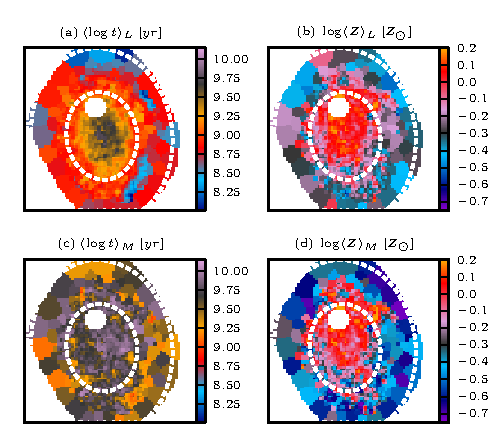
\includegraphics{figuras/at-aZ-K0277}
	\caption[Idade estelar e metalidade espacialmente resolvidas para a
	galáxia NGC 2916] {Idade e metalicidade estelar média, espacialmente
	resolvidas, para a galáxia NGC 2916. (a) Idade estelar média pesada pela
	luminosidade. (b) metalicidade estelar média pesada pela luminosidade.
	(c) Idade estelar média pesada pela massa. (d) metalicidade estelar
	média pesada pela massa. Retirado de
	\citet[figura 6]{CidFernandes2013}, Apêndice \ref{apendice:PaperResolving1}.}
	\label{fig:ataZMap}
\end{figure}

\begin{figure}
	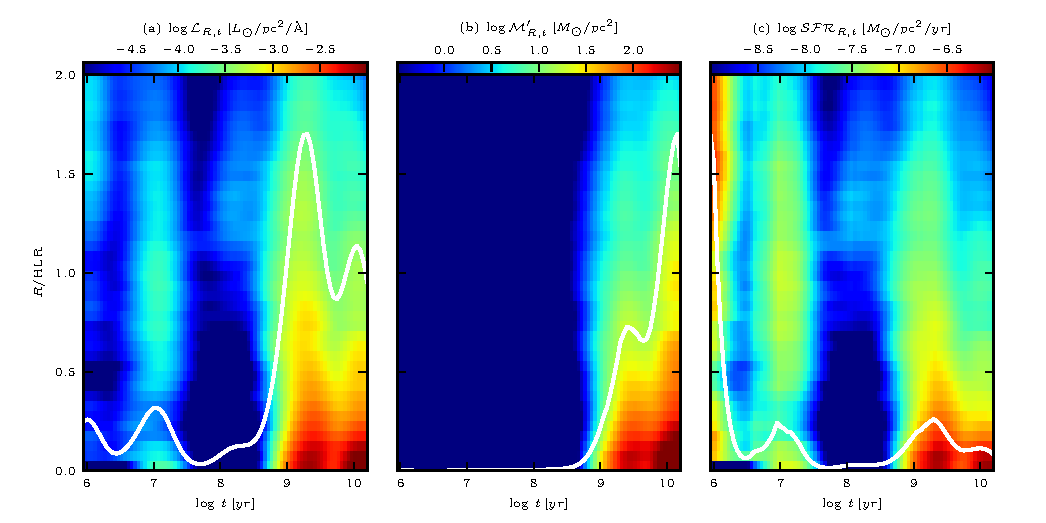
\includegraphics[width=1.0\columnwidth]{figuras/L-M-SFR-K0277}
	\caption[Diagramas $R \times t$ para luz, massa e SFR] {Diagramas $R \times t$
	para luz, massa e taxa de formação estelar (SFR). (a) Luminosidade em
	$5635\,\angstrom$ por unidade de área.  (b) Massa transformada em estrelas por
	unidade de área. (c) Taxa de formação estelar por unidade de área. A linha
	sólida representa o gráfico colapsado na direção vertical, apenas para ilustrar
	a variação temporal das quantidades mapeadas. Retirado de
	\citet[figura 12]{CidFernandes2013}, Apêndice \ref{apendice:PaperResolving1}.}
	\label{fig:LMSFR2D}
\end{figure}

As Figuras \ref{fig:LMAVMap} e \ref{fig:ataZMap} mostram mapas de propriedades
físicas obtidas pela síntese espectral. Propriedades como a massa (Figura
\ref{fig:LMAVMap}d) e luminosidade (Figuras \ref{fig:LMAVMap}a e
\ref{fig:LMAVMap}c) são quantidades extensivas, e são proporcionais à escala. Já
a atenuação por poeira (Figura \ref{fig:LMAVMap}b), idade e metalicidade estelar
são quantidades intensivas, independentes de escala. Na prática isto significa
que as quantidades extensivas podem ser divididas entre os {\em pixels} que
compõem uma zona, enquanto as intensivas são uma propriedade comum a todos os
{\em pixels} desta zona. Esta diferença pode ser notada nas zonas mais externas
dos mapas, onde aparecem platôs na quantidades intensivas. As quantidades
extensivas passam por um processo apelidado de ``dezonificação'', onde uma
medida referente a uma zona é dividida entre os {\em pixels} com base em um
peso, normalmente dado pelo fluxo na janela de normalização. Isto faz com que as
imagens não tenham um aspecto segmentado, com patamares nas zonas periféricas.

Um dos desafios de se trabalhar com cubos multidimensionais é como visualizar
esta informação. Uma alternativa é comprimir determinadas dimensões. Para
ilustrar esta capacidade do PyCASSO, a Figura \ref{fig:LMSFR2D} mostra diagramas
de luz, massa e taxa de formação estelar (SFR) em função do tempo, onde as
dimensões $x$ e $y$ foram transformadas em distância radial. Diagramas como
este, junto com perfis 1-D radiais e temporais ajudam a visualizar e interpretar
o resultado da síntese espectral, oferecendo novas ferramentas para estudar a
estrutura e evolução de galáxias.


%***************************************************************%
%                                                               %
%       PyCASSO - Resolving galaxies in Space and Time II       %
%                                                               %
%***************************************************************%

\subsection{Artigo: {\em Resolving galaxies in time and space: II: Uncertainties
in the spectral synthesis of datacubes}}
\label{sec:pycasso:art:Resolving2}

Uma crítica bastante comum aos métodos de ajuste é que eles não provêm a
incerteza associada aos valores ajustados. A forma mais simples de determinar
esta incerteza é refazer o ajuste várias vezes, perturbando as medidas levando
em conta os erros de forma realista. Este artigo por \citet{CidFernandes2013}
investiga a incerteza nos ajustes feitos no artigo discutido na seção anterior.
O artigo está reproduzido na íntegra no Apêndice \ref{apendice:PaperResolving2}.

Quando se injetam erros aleatórios, obtém-se incertezas de $\sim
0.08\,\mathrm{dex}$ em idades e metalicidades pesadas pela luminosidade, e de
$\sim 0.15\,\mathrm{dex}$ quando pesadas pela massa. A massa estelar teve uma
incerteza de $\sim 0.08\,\mathrm{dex}$, e $A_V$ de $\sim 0.06\,\mathrm{mag}$.
Injetando erros sistemáticos em cor\footnote{Adicionando componentes lineares em
comprimento de onda, a fim de emular uma má calibração de fluxo.} as incertezas
são similares, exceto para $A_V$, que recebe um desvio sistemático de
$+0.05\,\mathrm{mag}$ e uma incerteza de $\sim 0.16\,\mathrm{mag}$.

\begin{figure}
	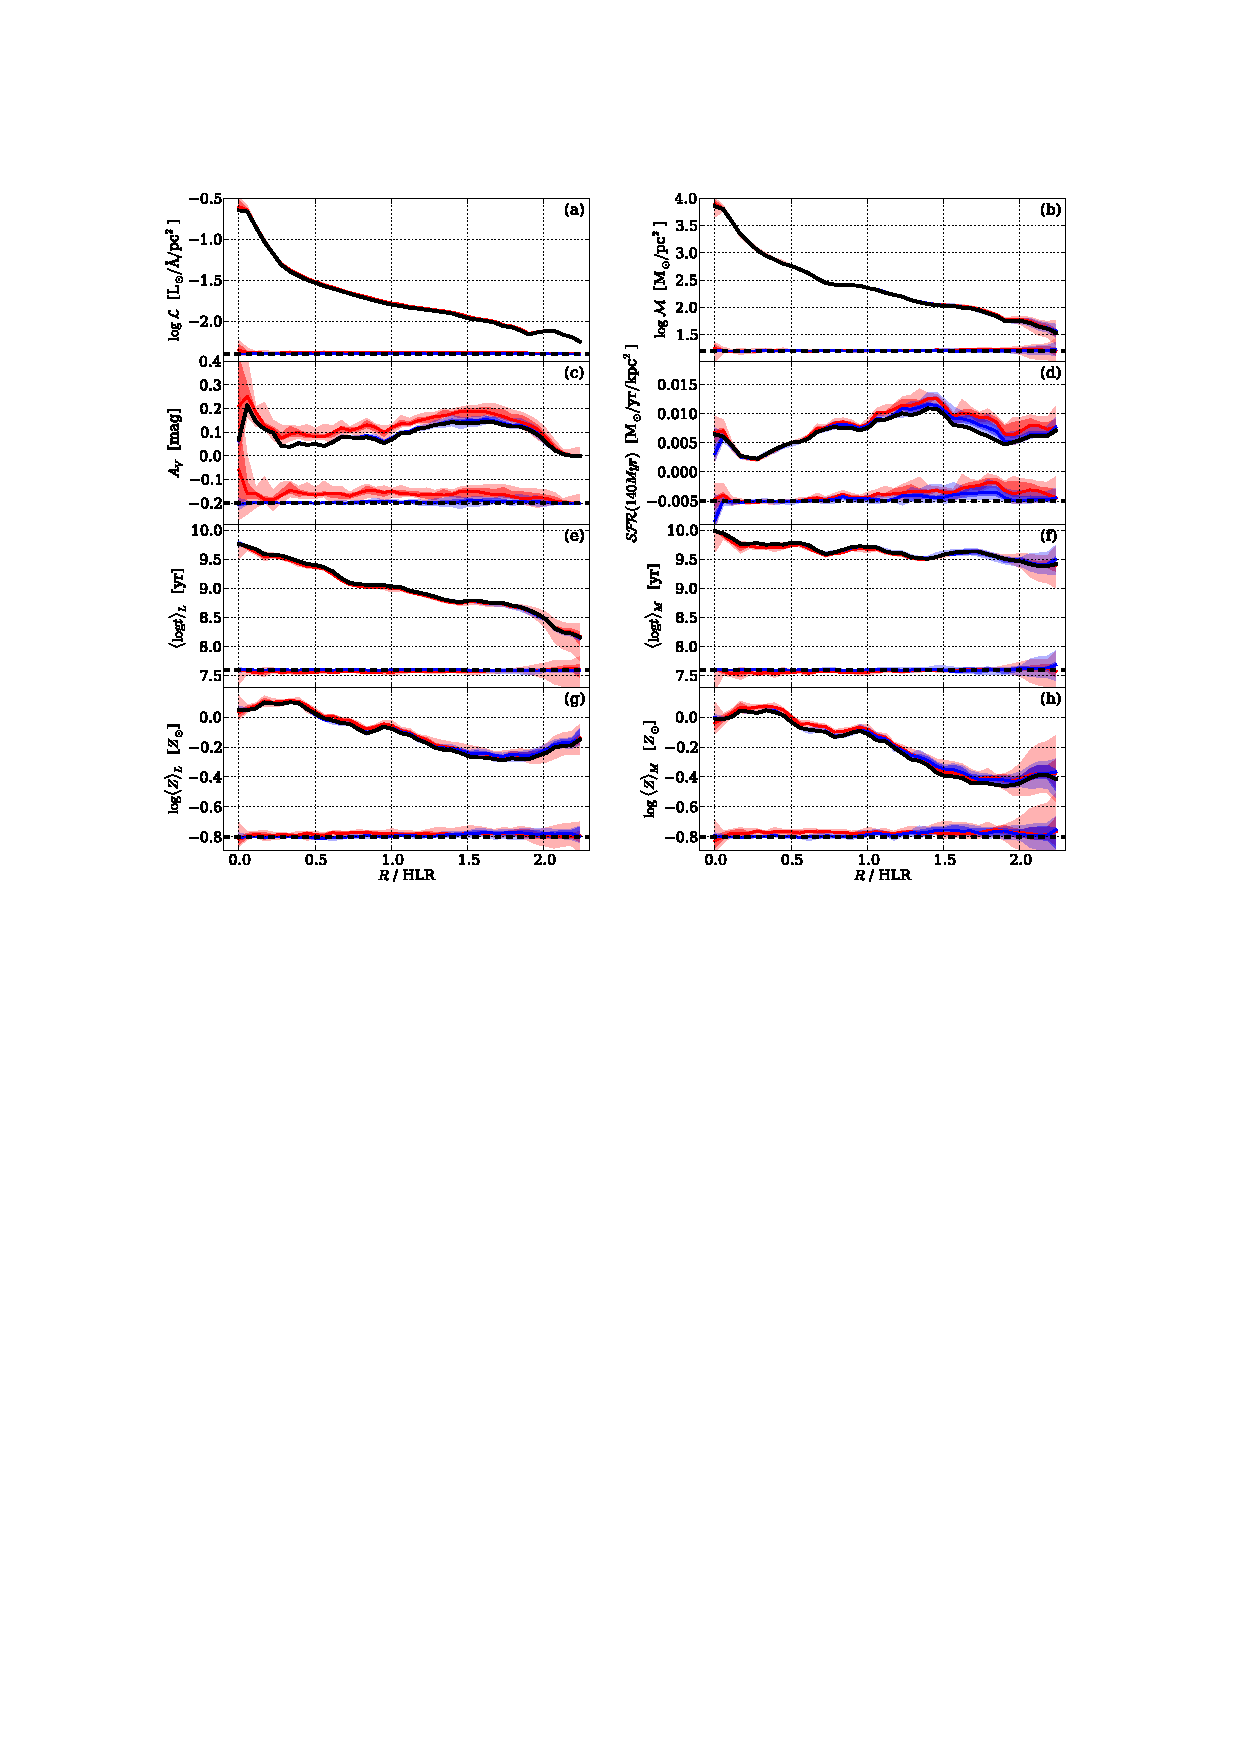
\includegraphics[width=1.0\columnwidth]{figuras/resolving2}
	\caption[Incerteza nos perfis radiais] {Incerteza nos perfis radiais de
	algumas propriedades. (a) Luminosidade superficial a $5635\,\angstrom$,
	corrigida de extinção. (b) Densidade superficial de massa. (c) Atenuação na
	banda $V$. (d) Taxa de formação estelar (últimos $140\, \mathrm{Ma}$) por
	unidade de área. (e) Idade estelar média ponderada pela luminosidade. (f) Idade
	estelar média ponderada pela massa. (g) Metalicidade estelar média ponderada
	pela luminosidade. (h) Metalicidade estelar média ponderada pela massa. As
	linhas em preto marcam a solução original. Em faixas azuis e vermelhas, as
	distribuições das realizações com ruído aleatório, e sistemático em cor,
	respectivamente. A diferença entre as simulações e o original está desenhada
	abaixo de cada painel, com o zero marcado pela linha tracejada. Retirado de
	\citet[figura 4]{CidFernandes2014}, Apêndice \ref{apendice:PaperResolving2}.}
	\label{fig:incertRad}
\end{figure}

Embora haja uma incerteza considerável analisando-se as propriedades da galáxia
pixel a pixel, os perfis radiais em geral são bastante robustos. Propriedades
diretas como a luminosidade, massa, idade e metalicidade estelar, quando vistas
em perfil radial (Figura \ref{fig:incertRad}), mantêm o mesmo formato com pouca
dispersão, exceto nas regiões mais afastadas do núcleo, onde há poucas zonas. Na
verdade, qualquer forma de média espacial que envolva {\em pixels} (ou zonas)
suficientes deverá levar a uma diminuição na incerteza.

\begin{figure}
	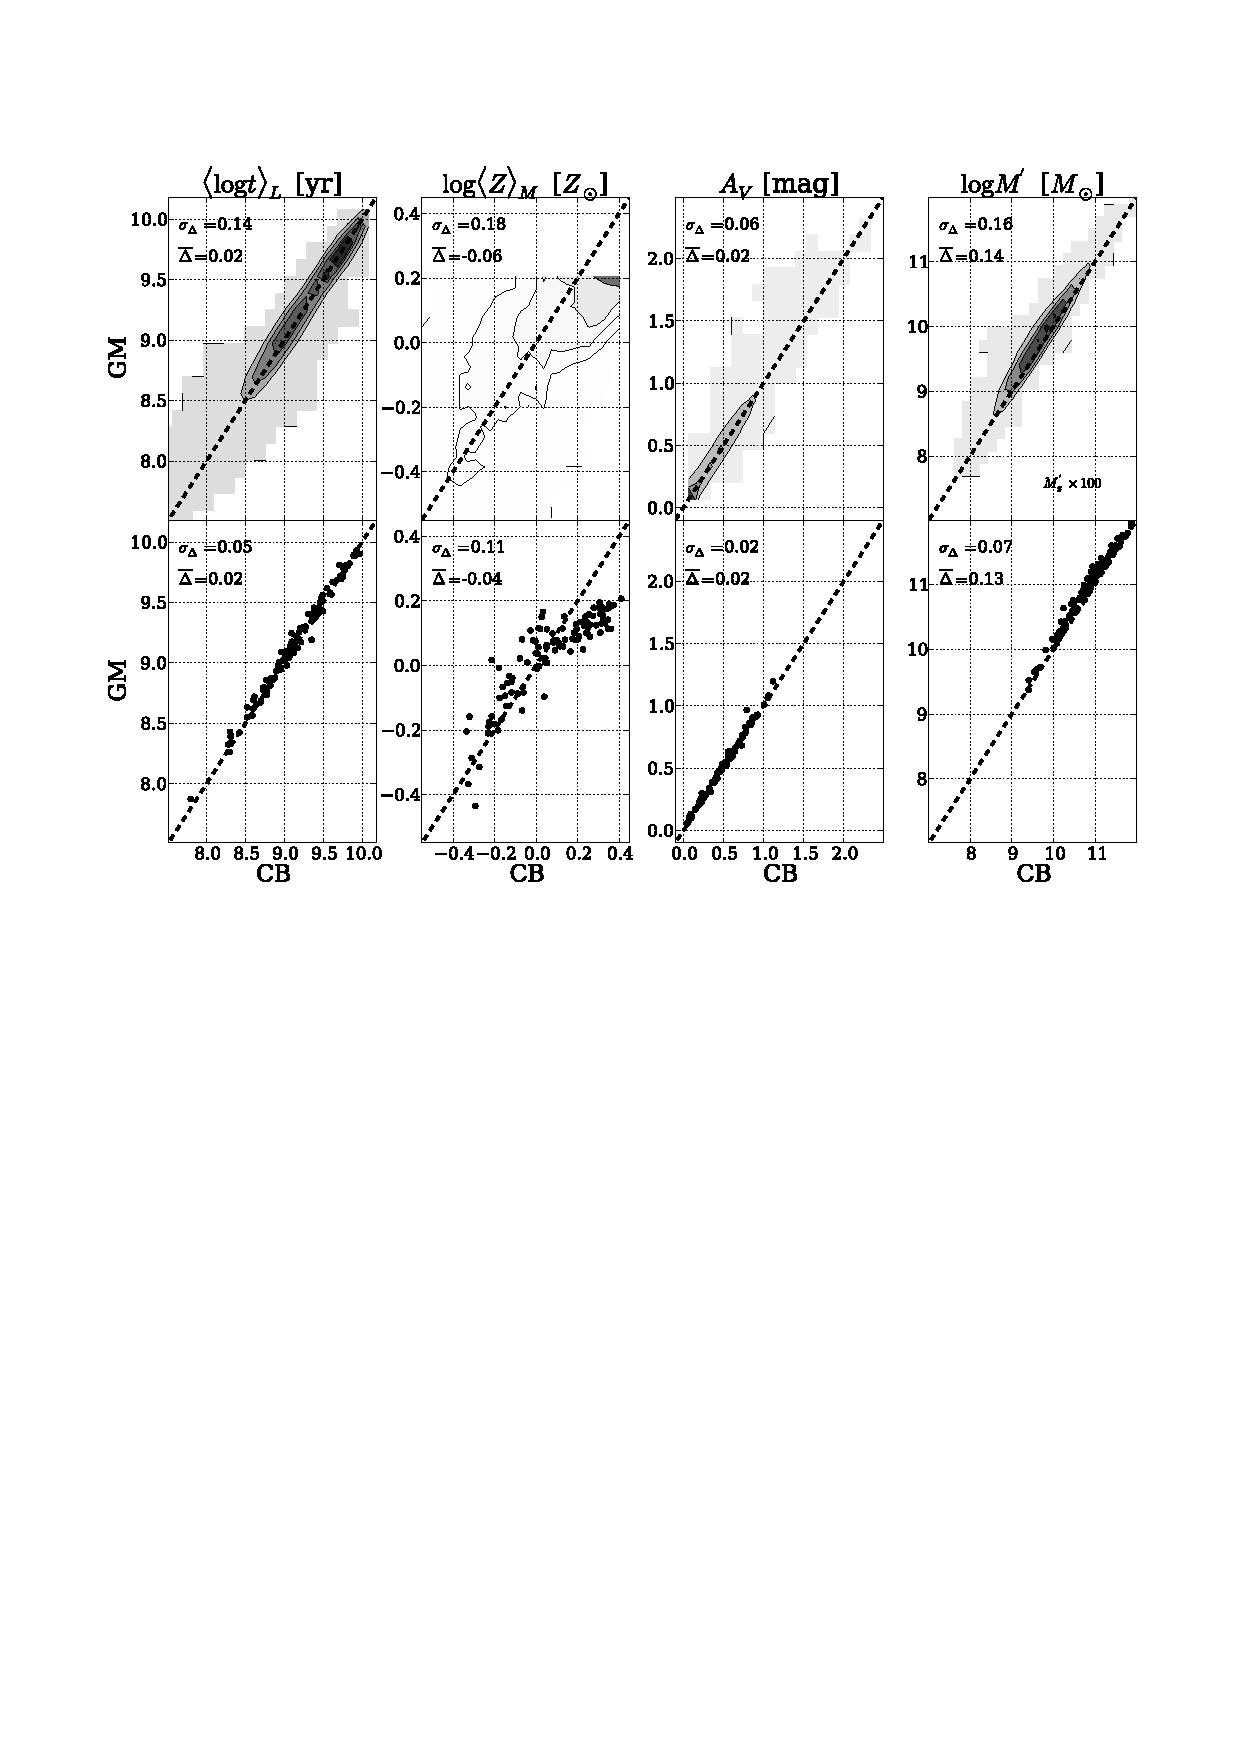
\includegraphics[width=1.0\columnwidth]{figuras/resolving2-base}
	\caption[Comparação dos ajustes com bases de SSP diferentes]
	{Comparação de propriedades obtidas com o ajuste utilizando as bases
	GM (eixo vertical) CB (eixo horizontal). Os painéis superiores mostram um
	histograma 2-D com contornos para propriedades de cada pixel de 107 galáxias do
	CALIFA. Da esquerda para a direita: idade estelar ponderada pela luminosidade,
	metalicidade estelar ponderada pela massa, atenuação na banda $V$, massa
	estelar inicial. Os painéis inferiores mostram a distribuição das mesmas
	propriedades, porém calculadas para o espectro integradas das galáxias.
	Retirado de \citet[figura 9]{CidFernandes2014}, Apêndice
	\ref{apendice:PaperResolving2}.}
	\label{fig:incertRad-base}
\end{figure}

O artigo também explora os efeitos da escolha da base de SSPs nos resultados do
ajuste. Em geral, bases diferentes levam a resultados consistentes.
Pode-se ver na Figura \ref{fig:incertRad-base} que a idade estelar
média ponderada pela luminosidade, a atenuação e a massa estelar inicial
têm uma concordância muito boa entre as bases. As metalicidades médias mostram
uma correlação, mas com uma dispersão muito grande, certamente devido a
diferenças nas trajetórias evolucionárias dos modelos, poucos valores
de metalicidade na base, e diferenças na metalicidade máxima da base. A
incerteza nestas propriedades mencionadas acima é cerca de $2$ vezes maior do
que as calculadas adicionando ruído aleatório. Claramente a escolha de uma base
adequada é de grande importância para a análise.


%***************************************************************%
%                                                               %
%                 PyCASSO - Inside-out growth                   %
%                                                               %
%***************************************************************%

\subsection{Artigo: {\em The Evolution of Galaxies Resolved in Space and Time: A
View of Inside-out Growth from the CALIFA Survey}}
\label{sec:pycasso:art:InsideOut}

Em \citet{Perez2013} se estuda o crescimento de dentro para fora de $105$
galáxias do CALIFA. O estudo se baseia na síntese espectral com o \starlight, e
segue exatamente a mesma prescrição de \citet{CidFernandes2014}, descrita na
Seção \ref{sec:pycasso:art:Resolving1}. O artigo está reproduzido na íntegra no
Apêndice \ref{apendice:InsideOut}.

Galáxias vêm em todos os tamanhos. Para determinar o crescimento, as distâncias
são normalizadas utilizando o raio onde a luminosidade cumulativa (em
$5635\,\angstrom$) alcança $50\%$ da luminosidade total da galáxia, denominado
$R_{50}$ (ou HLR\footnote{{\em Half Light Radius}.}). As galáxias da amostra são
separadas em caixas com $15$ galáxias cada, segundo a sua massa. O crescimento
em massa em função do tempo é calculado para cada pixel de cada galáxia e somado
em cada caixa de massa.

\begin{figure}
	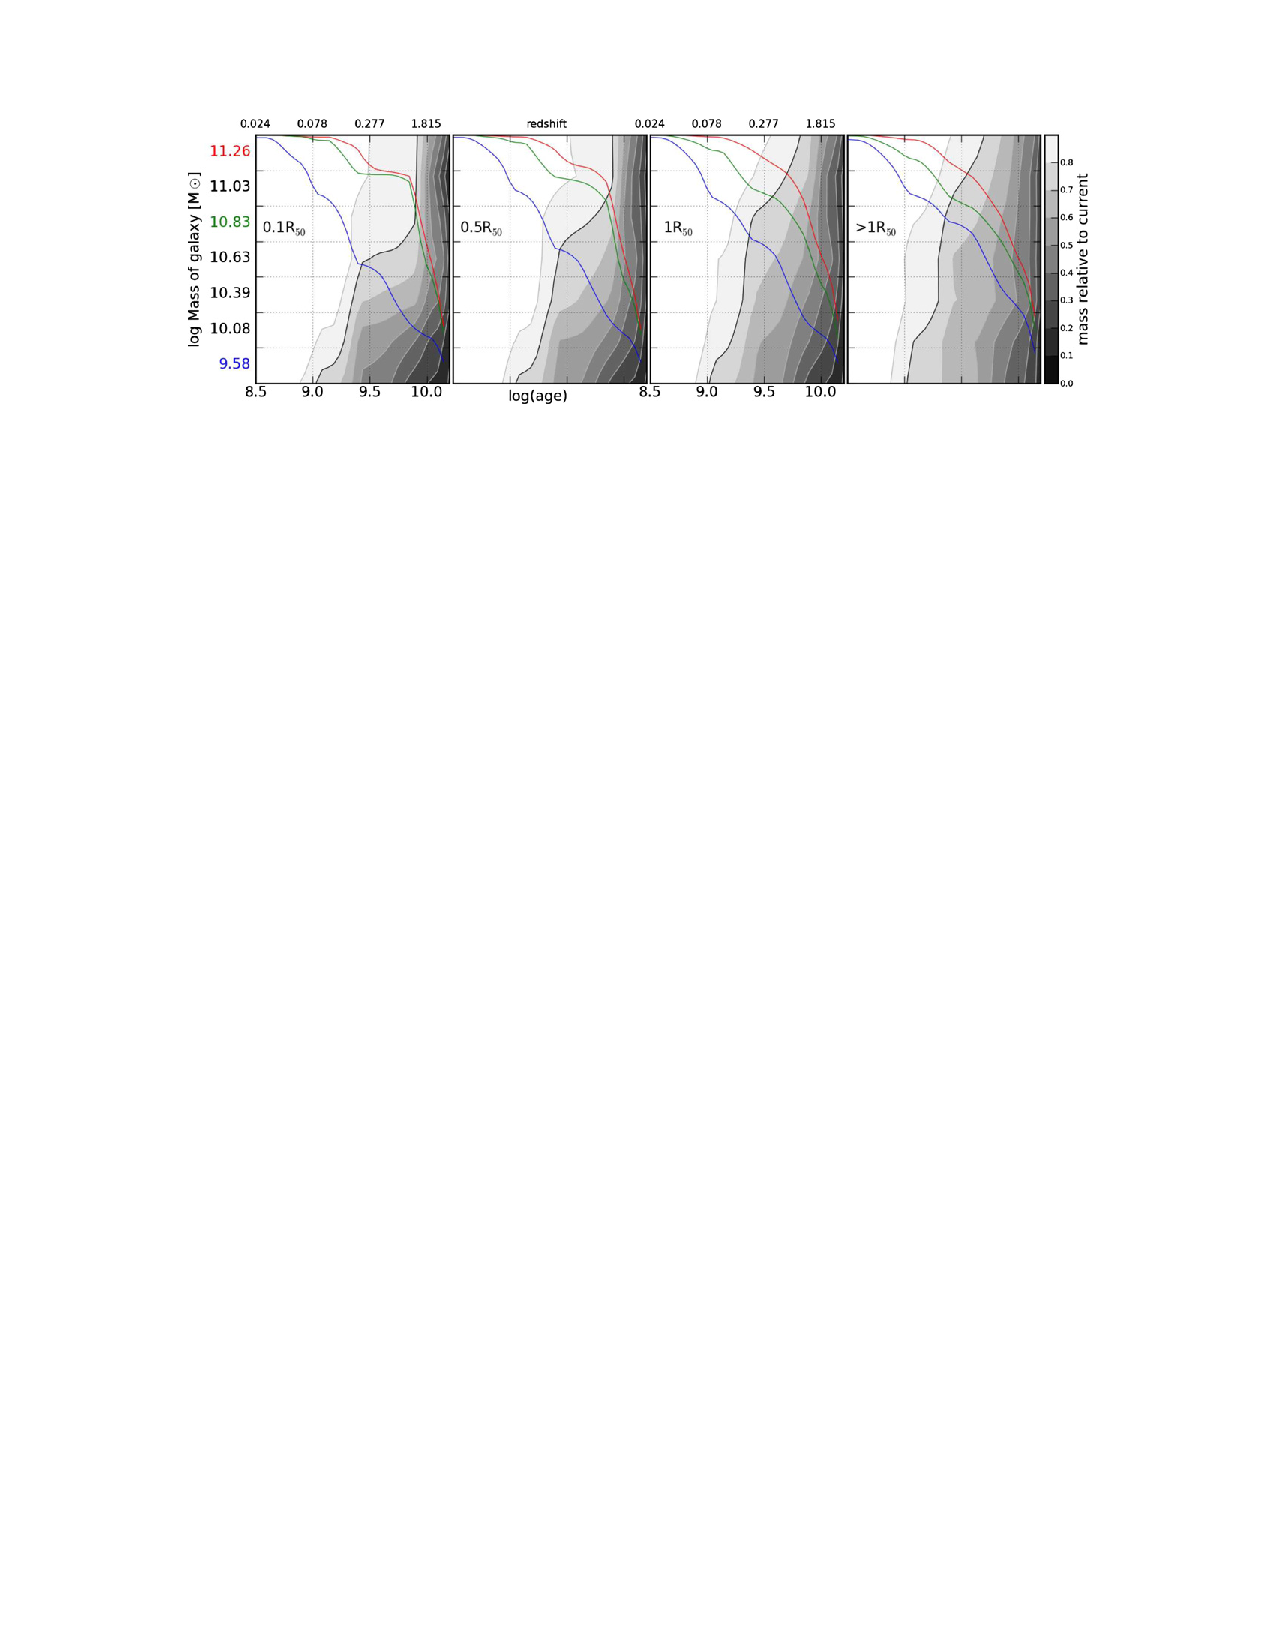
\includegraphics{figuras/inside-out}
	\caption[Crescimento da massa estelar de galáxias de dentro para fora]
	{Crescimento de massa estelar de dentro para fora. As $105$ galáxias foram
	separadas em grupos de 15, em massa, formando as caixas do eixo vertical.
	Os painéis mostram o crescimento da massa em escala de cinza, normalizado, em
	função do tempo e da massa das galáxias. O contorno em preto marca $80\%$. Da
	direita para a esquerda se vê as regiões em raio $r < 0,1\,R_{50}$, $0,1 < r
	\leq 0,5\,R_{50}$, $0,5 < r \leq 1\,R_{50}$ e $r > 1\,R_{50}$. Para
	facilitar a visualização da forma da variação temporal, as linhas azuis, verdes
	e vermelhas em cada painel mostram um corte horizontal nas caixas inferior,
	intermediário e superior, com escala de $0$ a $1$. Retirado de \citet[figura
	9]{Perez2013}, Apêndice \ref{apendice:InsideOut}.}
	\label{fig:insideOut}
\end{figure}

A Figura \ref{fig:insideOut} ilustra o crescimento de massa em anéis crescentes
em raio ($0,1\,R_{50}$, $0,5\,R_{50}$, $1\,R_{50}$ e $>1\,R_{50}$.). Em cada
painel, o tempo passa da direita para a esquerda, e a massa estelar,
normalizada, cresce desde zero (direita, em preto) até $1$ (esquerda, em
branco). Se vê claramente que galáxias menos massivas, na parte inferior das
figuras, têm um crescimento gradual mais ou menos constante em todos os raios.
As galáxias mais massivas, na parte superior das figuras, apresentam um
crescimento muito rápido nas regiões centrais, enquanto as regiões externas
crescem mais gradualmente. As linhas azul, verde e vermelha, em cada painel,
representam cortes horizontais na caixa de mais baixa massa, no intermediário e
no de mais alta massa, respectivamente, para facilitar a visualização. A mudança
de regime ocorre em $\log M_\star = 10,83$, ou seja, uma massa de $\sim
7\times10^{10}\,M_\odot$. Vários estudos indicam esta faixa como uma ``massa
especial'', onde a taxa de formação estelar alcança valores altos muito
rapidamente. De qualquer forma, esta é uma evidência observacional de algo que
já se suspeita há muito tempo: que as galáxias massivas se formaram de dentro
para fora.


%***************************************************************%
%                                                               %
%                 PyCASSO - Radial structures                   %
%                                                               %
%***************************************************************%

\subsection{Artigo: {\em The star formation history of CALIFA galaxies: Radial
structures}}
\label{sec:pycasso:art:RadStruct}

O artigo por \citet{GonzalezDelgado2014a} faz um estudo detalhado da estrutura
radial de diversas propriedades de $107$ galáxias do CALIFA. O artigo está
reproduzido na íntegra no Apêndice \ref{apendice:RadStruct}.
Um dos resultados mais importantes é que a densidade superficial de massa
estelar e idade estelar média ponderada por luminosidade, medidas a $1\,R_{50}$,
são representativos das médias da galáxia como um todo. A Figura
\ref{fig:radStruct1} mostra a correlação entre os valores em três raios
distintos e o global para a idade estelar média ponderada pela luminosidade
(esquerda) e a densidade superficial de massa estelar (centro). Valores a
$1\,R_{50}$, marcado como HLR nas figuras, coincidem em geral com a média global
da galáxia.
Ainda na mesma figura pode-se ver a correlação entre a densidade superficial de
massa estelar média da galáxia e a massa estelar total da galáxia. Este
resultado está de acordo com \citet{Kauffmann2003}, usando a amostra do SDSS.

\begin{figure}
	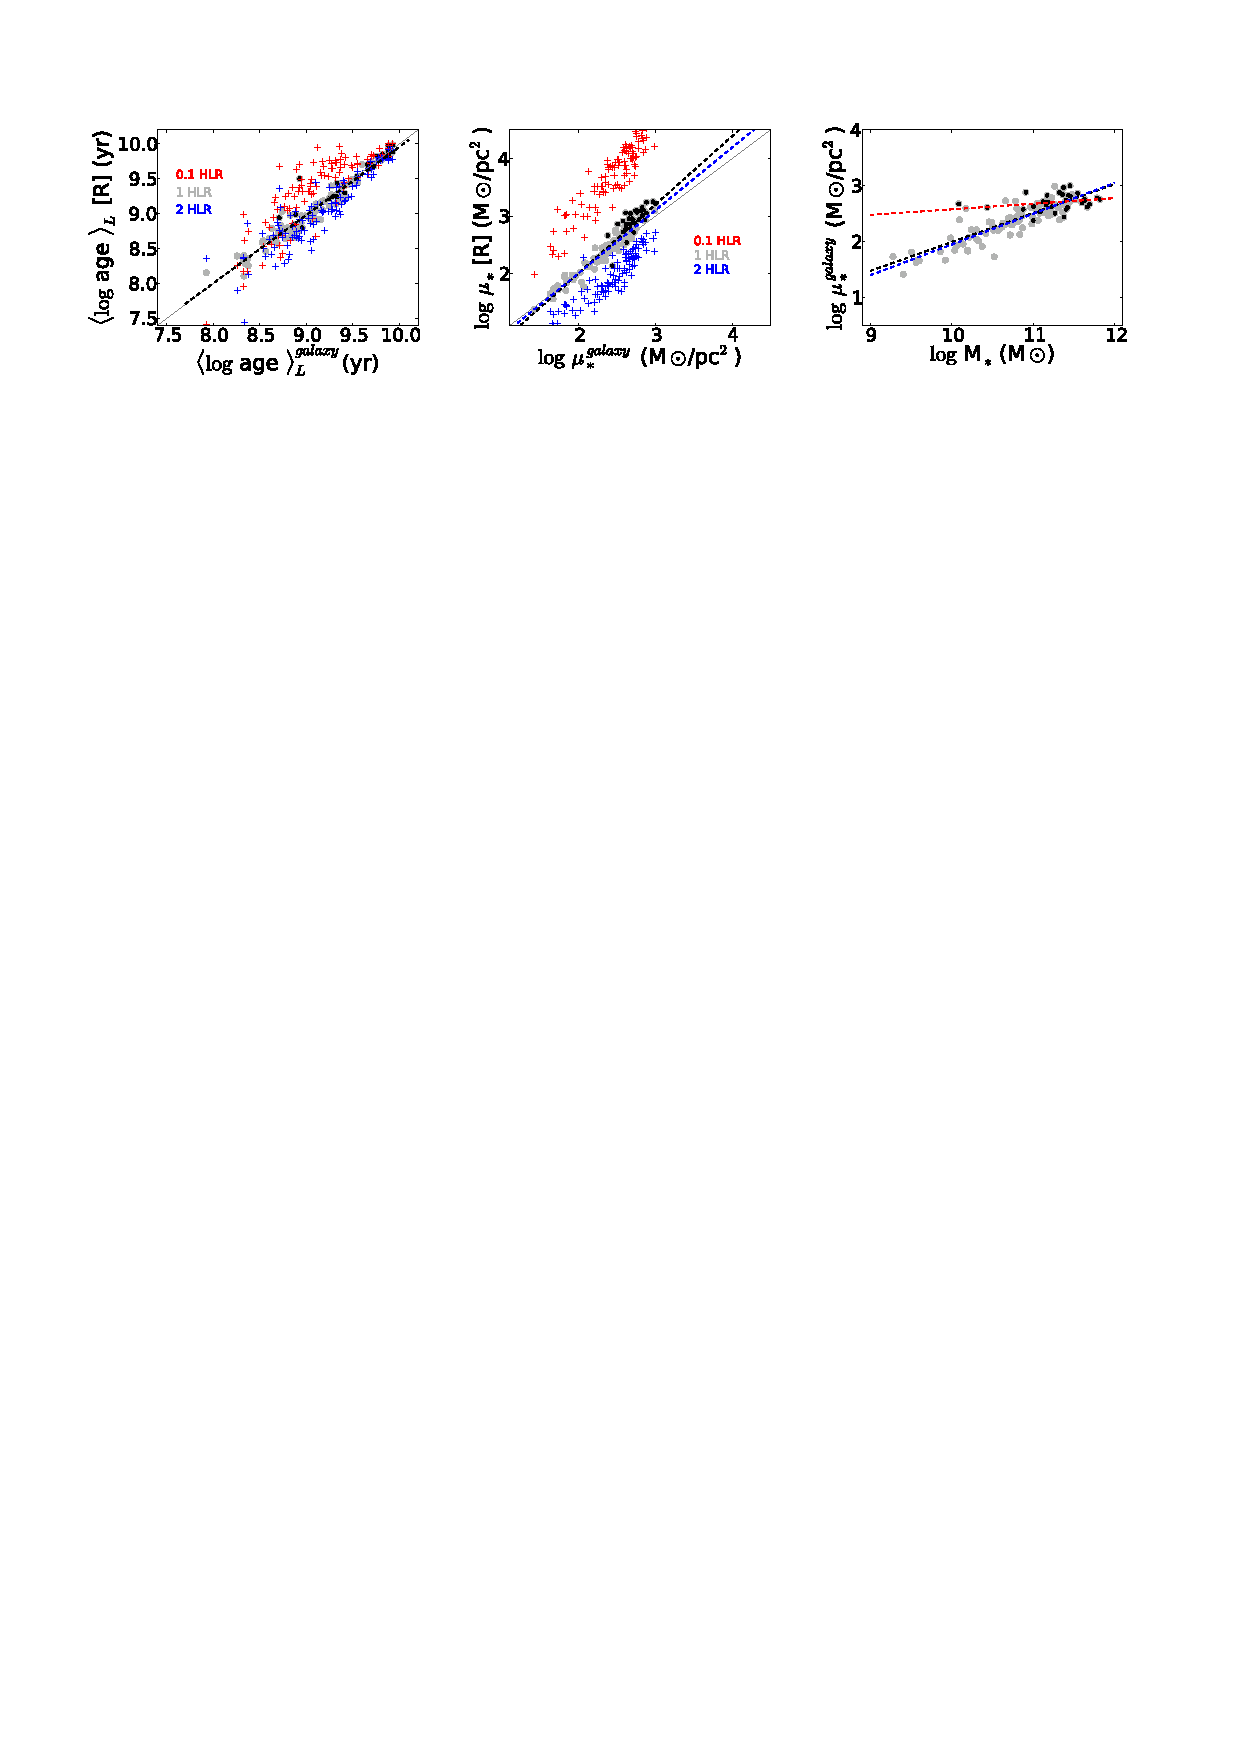
\includegraphics[width=1.0\columnwidth]{figuras/radstruct-01}
	\caption[Correlação entre idade, desidade superficial e massa estelar total]
	{Esquerda: correlação entre a idade estelar média ponderada pela luminosidade
	em $1\,R_{50}$ (círculos cinza), $0,1\,R_{50}$ (cruzes azuis), $2\,R_{50}$
	(cruzes vermelhas) e a média da galáxia. Pontos em preto marcam galáxias
	esferoidais, com $C \geq 2,8$. Meio: o mesmo gráfico para a densidade
	superficial de massa estelar. Direita: correlação entre a densidade
	superficial de massa média da galáxia e a massa estelar total da galáxia. As
	linhas tracejadas mostram o ajuste linear total (preto), apenas discos (azul),
	e apenas para esferoidais (vermelho).  Retirado de \citet[figura
	6]{GonzalezDelgado2014a}, Apêndice \ref{apendice:RadStruct}.}
	\label{fig:radStruct1}
\end{figure}

O raio contendo metade da massa estelar (HMR\footnote{{\em Half Mass Radius}.})
é em média 20\% menor que $R_{50}$ (HLR). A razão entre HMR e HLR tem correlação
com a massa total da galáxia e o tipo morfológico. Na Figura
\ref{fig:radStruct2} pode-se ver que a relação HMR/HLR diminui com a massa
estelar para galáxias com massa menor que $10^{11}\,M_\odot$, enquanto permanece
constante para galáxias mais massivas. Um comportamento similar ocorre com o
tipo morfológico:
em galáxias com disco a relação HMR/HLR diminui com a massa, e em galáxias
esferoidais a relação é aproximadamente constante.

\begin{figure}
	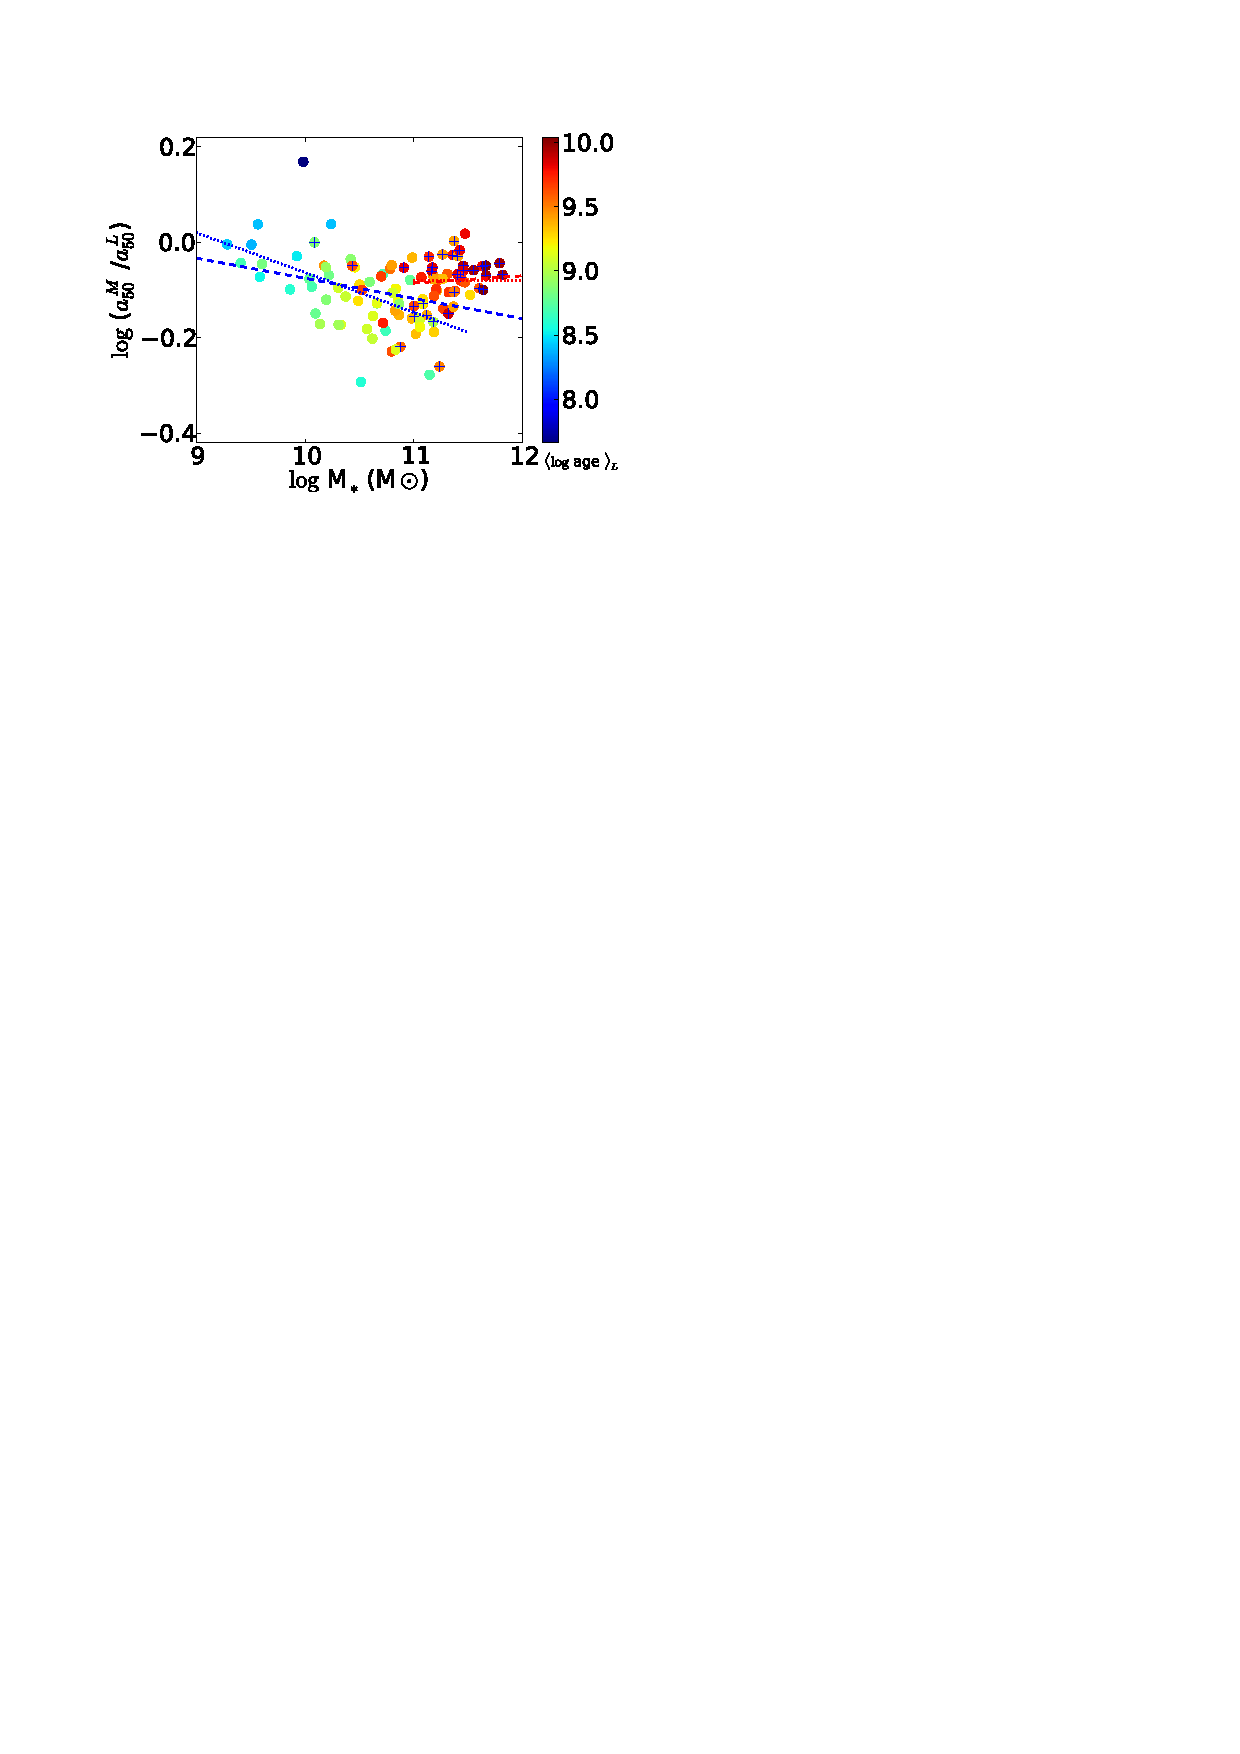
\includegraphics{figuras/radstruct-02}
	\caption[Relação entre $a^M_{50}/a^L_{50}$ e a massa estelar total]
	{Relação entre $a^M_{50}/a^L_{50}$ e a massa estelar total. A cor dos
	pontos reflete a idade estelar média ponderada pela luminosidade, em $0,5\,a^L_{50}$.
	Galáxias com índice de concentração $C \geq 2,8$ estão marcadas com uma cruz. A
	linha azul mostra o ajuste linear para galáxias com massa estelar. Retirado de
	\citet[figura 10]{GonzalezDelgado2014a}, Apêndice
	\ref{apendice:RadStruct}.}
	\label{fig:radStruct2}
\end{figure}

Para galáxias esferoidais, o gradiente de idade depende mais da massa estelar
total da galáxia do que da densidade superficial de massa estelar, que, conforme
o painel inferior esquerdo da Figura \ref{fig:radStruct3}, é aproximadamente
constante. A massa total da galáxia é a propriedade mais fundamental para
galáxias esferoidais, enquanto a densidade superficial de massa é mais
importante para as galáxias com disco.


\begin{figure}
	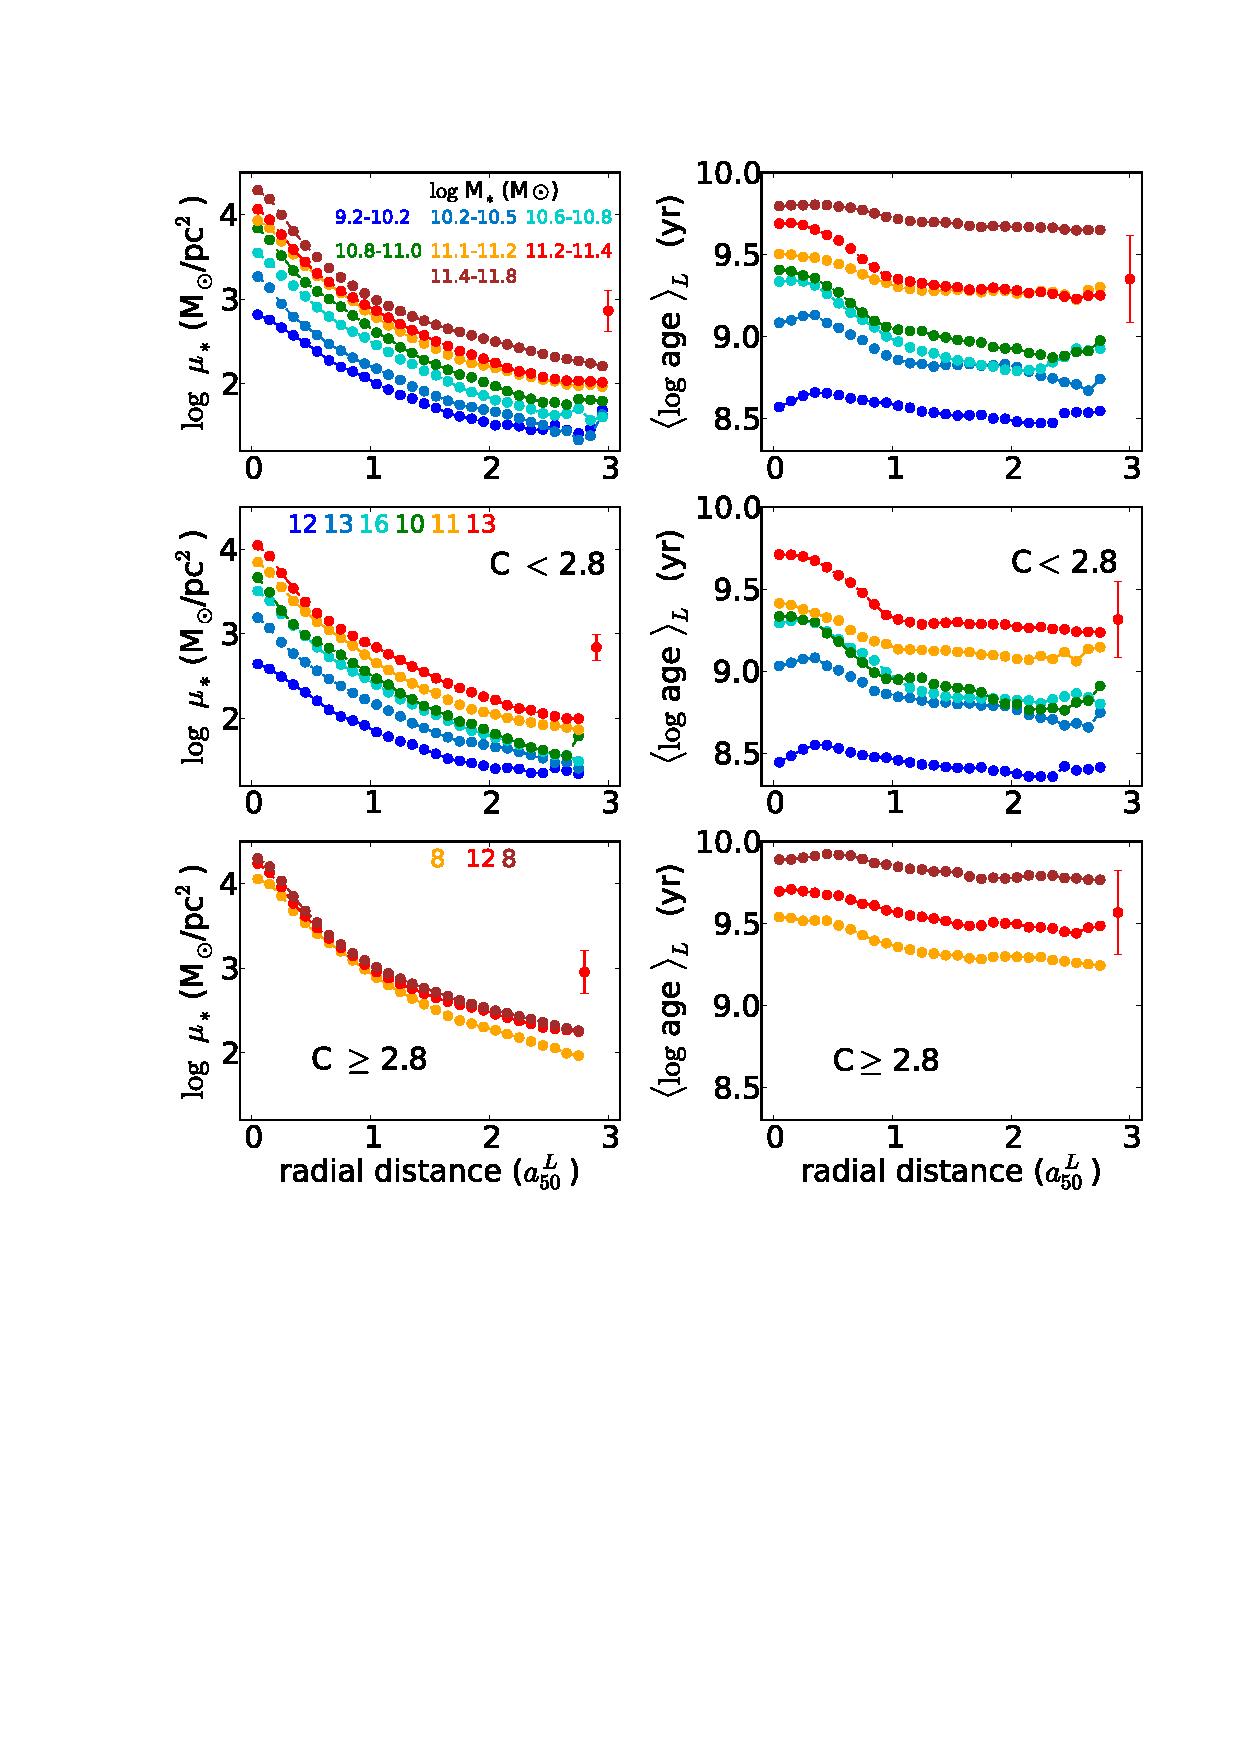
\includegraphics[width=0.8\columnwidth]{figuras/radstruct-03}
	\caption[Perfis radiais para várias caixas de massa estelar]
	{Perfis radiais da densidade superficial de massa estelar (esquerda) e idade
	estelar média ponderada pela luminosidade (direita), para caixas de
	massa estelar contendo 15 galáxias cada. Cima: todas as galáxias. As caixas
	em massa estão codificados em cores. Meio: galáxias dominadas por disco.
	Baixo: galáxias esferoidais ($C \geq 2,8$). Retirado de \citet[figura
	13]{GonzalezDelgado2014a}, Apêndice \ref{apendice:RadStruct}.}
	\label{fig:radStruct3}
\end{figure}

% FIXME: Rogério - Sugestões:
%
% * Qual a utilidade do pycasso nos papers?
% * Qual a tua participação em cada um dos artigos?
% * Quais as análises científicas que TU fizeste nestes artigos?

% End of this chapter
